Software guards our secrets, our money, our intellectual property,
our reputation \cite{covfefe}.  We entrust personal and
corporate information to software which works in an \emph{open} world, 
where  it interacts with % a vast number of
third party software of unknown provenance, possibly buggy and potentially malicious.

Thus, we expect and hope that our software will be \emph{robust}:
We expect and hope our software to behave correctly even if  used 
by erroneous or malicious third parties. Robustness means 
something different for each different software.
 We expect, \eg, that our bank will only make payments 
from our account if instructed by us or somebody authorized CITE-ERC20,
that  space on a web given to an advertiser will not be used
to obtain access to our bank details ... CITE-SOME-DOM-HORROR.

The importance of robustness has lead to the design of many programming
language mechanisms which help write robust programs:
constant fields or methods \cite{...}, private methods/fields\cite{...}, ownerschip\cite{...}
as well as the object capability paradigm\cite{millerPhDThesis},
and its adoption in  web systems
\cite{CapJavaHayesAPLAS17,CapNetSocc17Eide,DOCaT14} and programming languages such as Newspeak
\cite{newspeak17}, Dart \cite{dart15}, Grace \cite{grace,graceClasses}, Wyvern \cite{wyverncapabilities}.

While such programming language mechanisms make it \textit{possible} to write robust
programs, they cannot \textit{ensure} that programs are robust. 
To be able to do this, we need ways to specify what robustness means for the 
particular program, and ways to demonstrate that the particular program 
adheres to its specific robustness requirements.

There has been a plethora of work on the functional specification and verification of the
functional correctness of programs. Such specification describe what are
essentially \emph{sufficient} conditions for some
effect to happen. For example, if you make a payment request to your bank, money will be transferred
and as a result your funds will be reduced: the payment request is a sufficient condition for the
reduction of funds. However, a bank client is also interested in \emph{necessary} conditions:
they want to be assured that no reduction in their funds will take place unless they themselves
requested it.

Necessary conditions are essentially about things that will  \emph{not} happen. For example,
there  will be no reduction to the account's funds without the owner's explicit request: the request being made by
the owner is the necessary condition - under no other circumstances will the funds be reduced.

We give a visual representation of the difference between sufficient and necessary conditions in 
Fig. \ref{fig:NecessaryAndSuff}. We
represent the space of all theoretically possible behaviours as points in the rectangle, 
each function is a coloured oval and its possible behaviours are the points in the area of that oval.  
The sufficient conditions are described on a per-function basis. 
The necessary conditions, on the other hand are about the behaviour of a module as a whole, 
and describe what is guaranteed not to happen;
they are depicted as black triangles.

  \begin{figure}[htb]
 \begin{tabular}{ccccc}
\begin{minipage}{0.25\textwidth}
 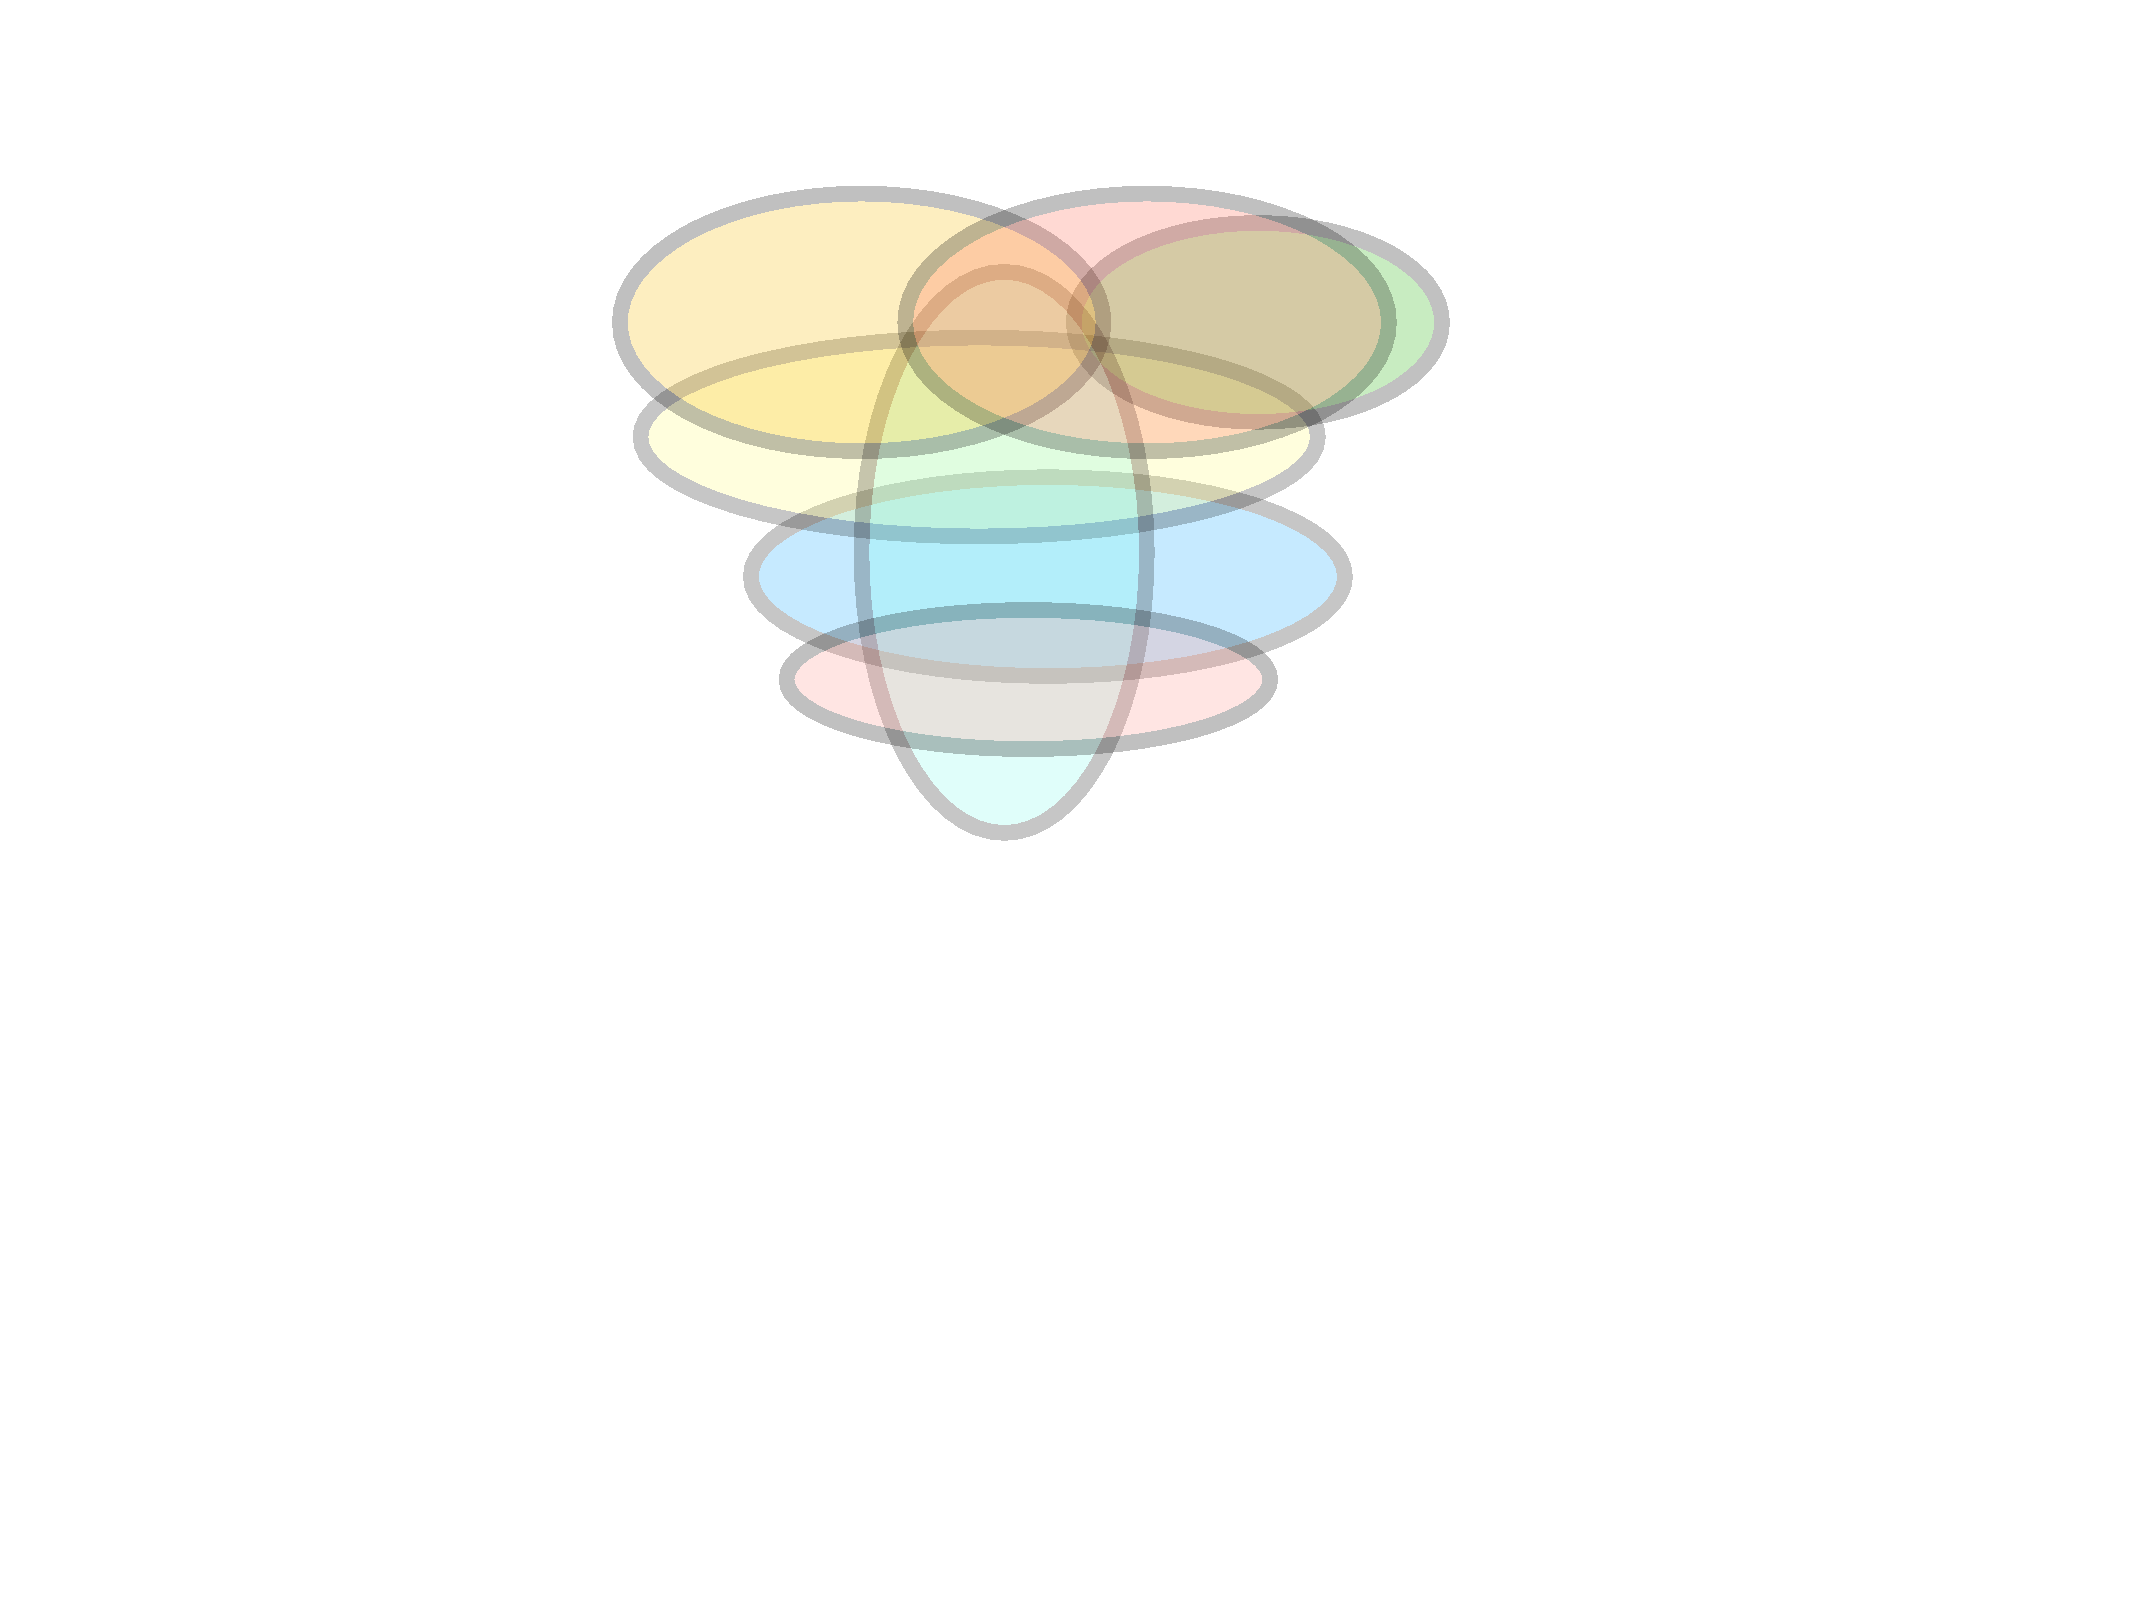
\includegraphics[width=\linewidth, trim=250  320 260 60,clip]{diagrams/Suff.pdf}
\end{minipage}
 & \ \ \ & 
\begin{minipage}{0.25\textwidth}
 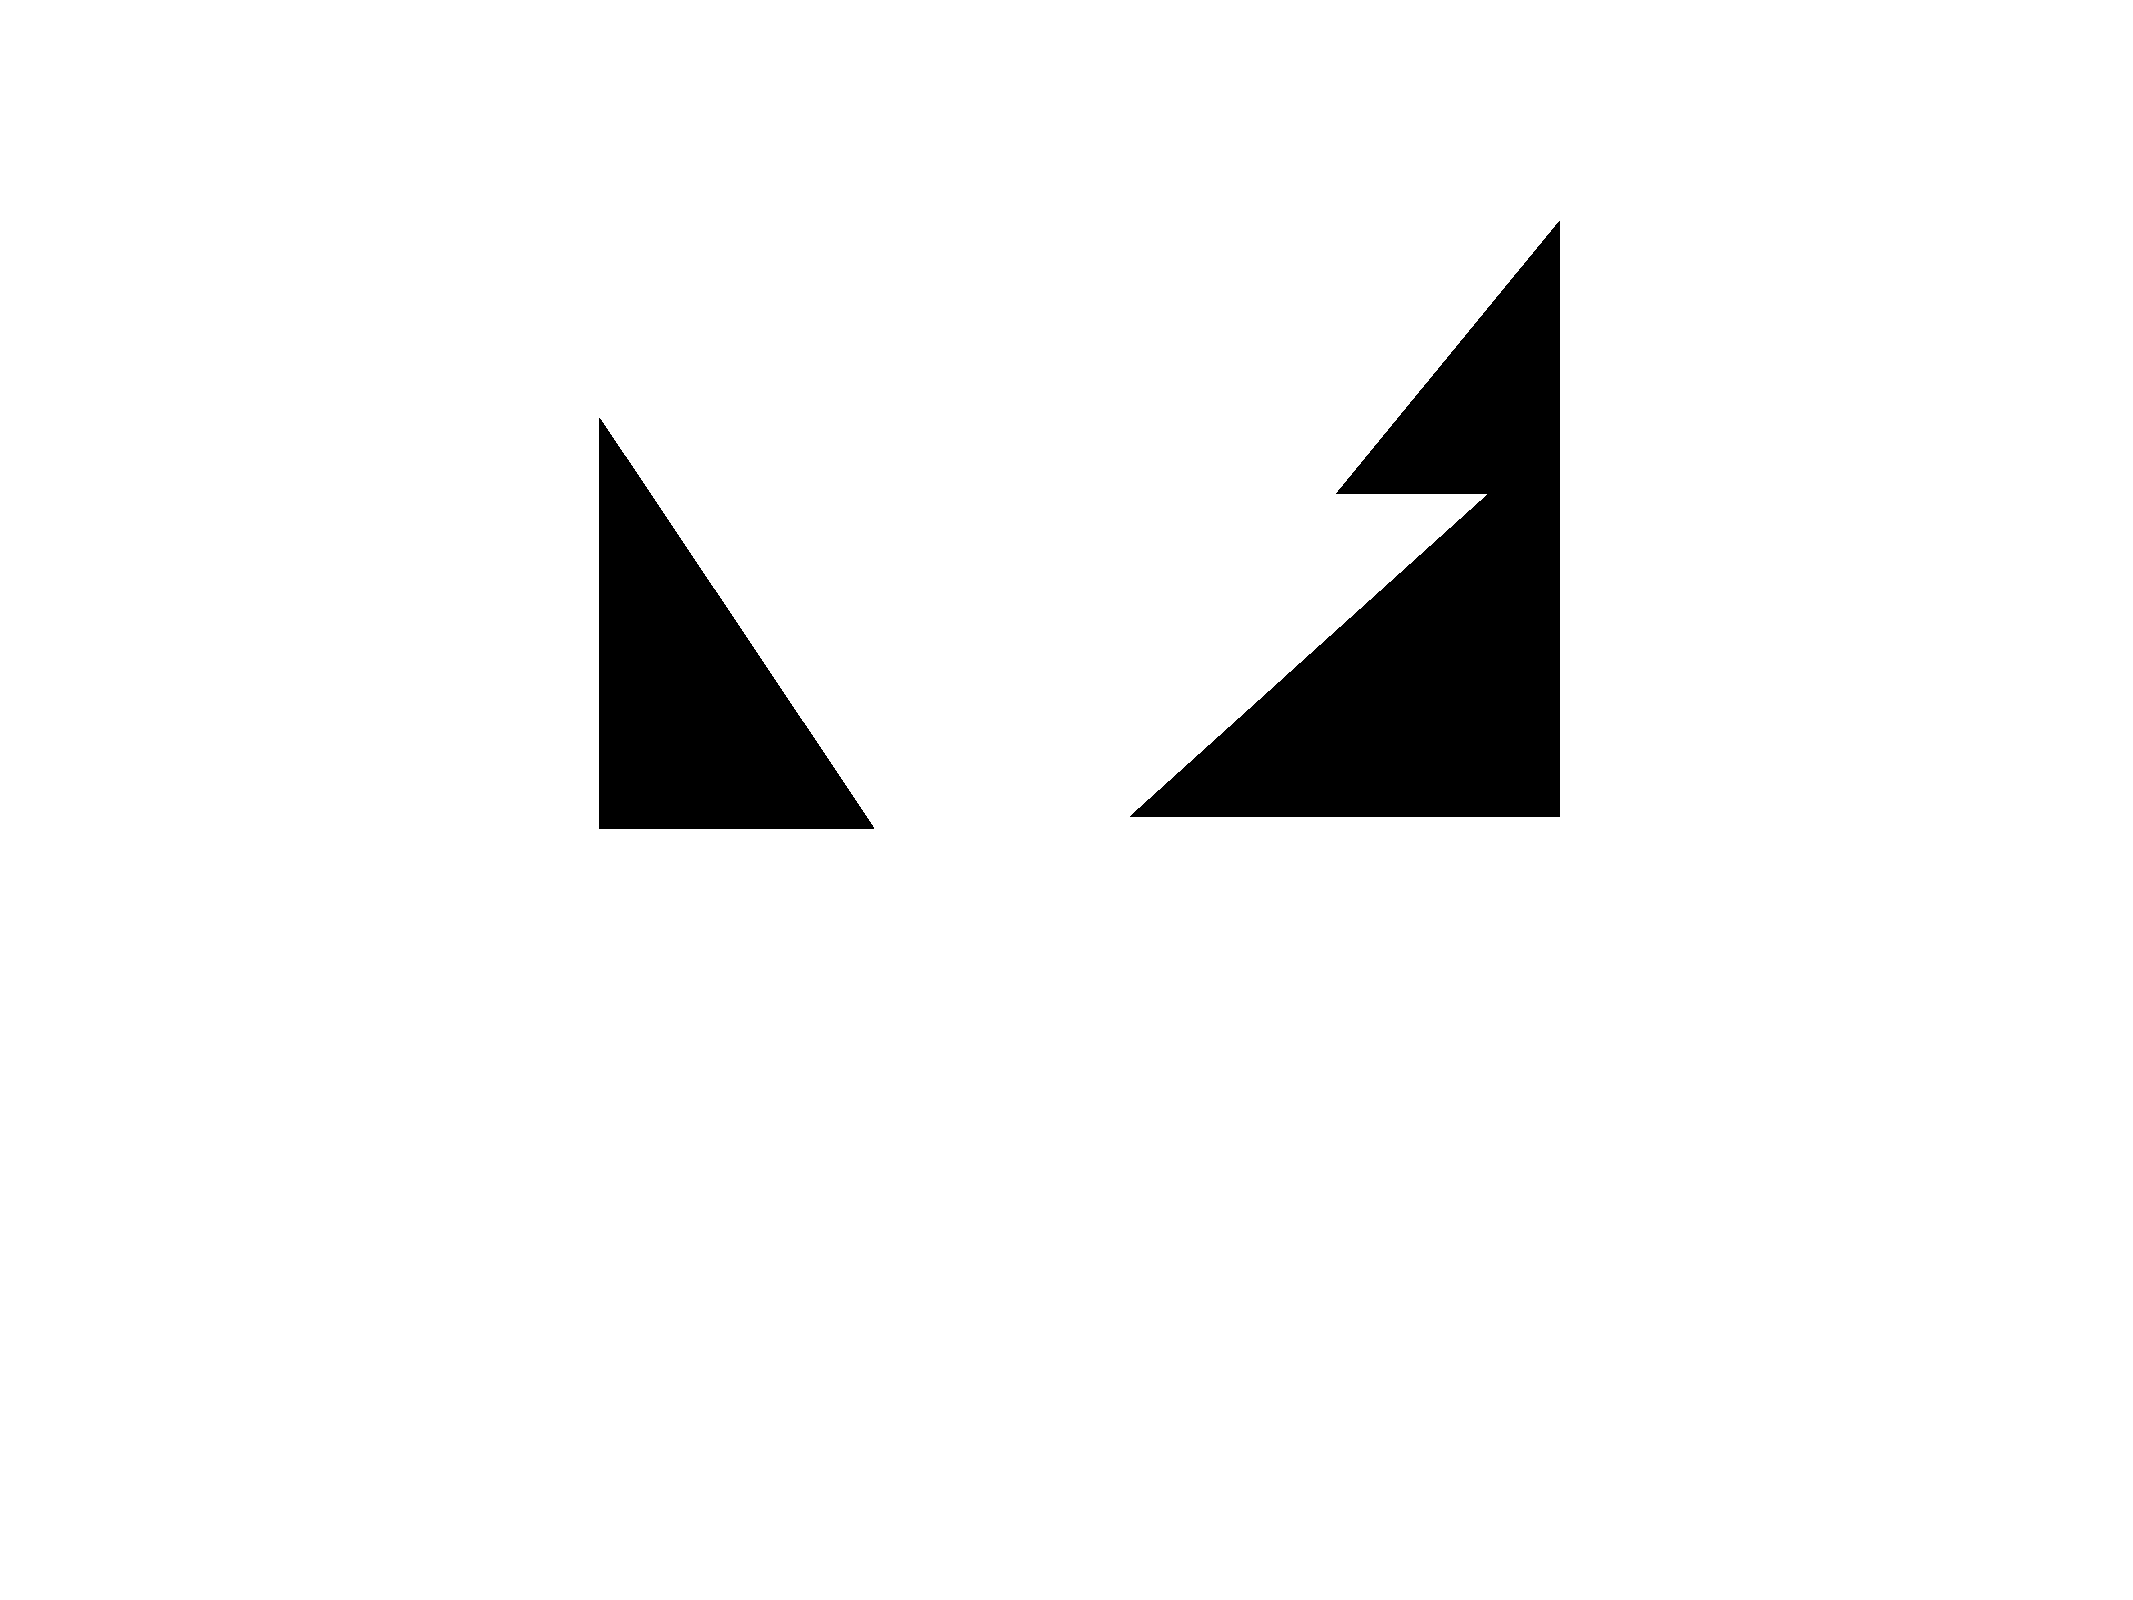
\includegraphics[width=\linewidth, trim=250  320 260 60,clip]{diagrams/Nec.pdf}
\end{minipage}
 & \ \ \ &
\begin{minipage}{0.25\textwidth}
 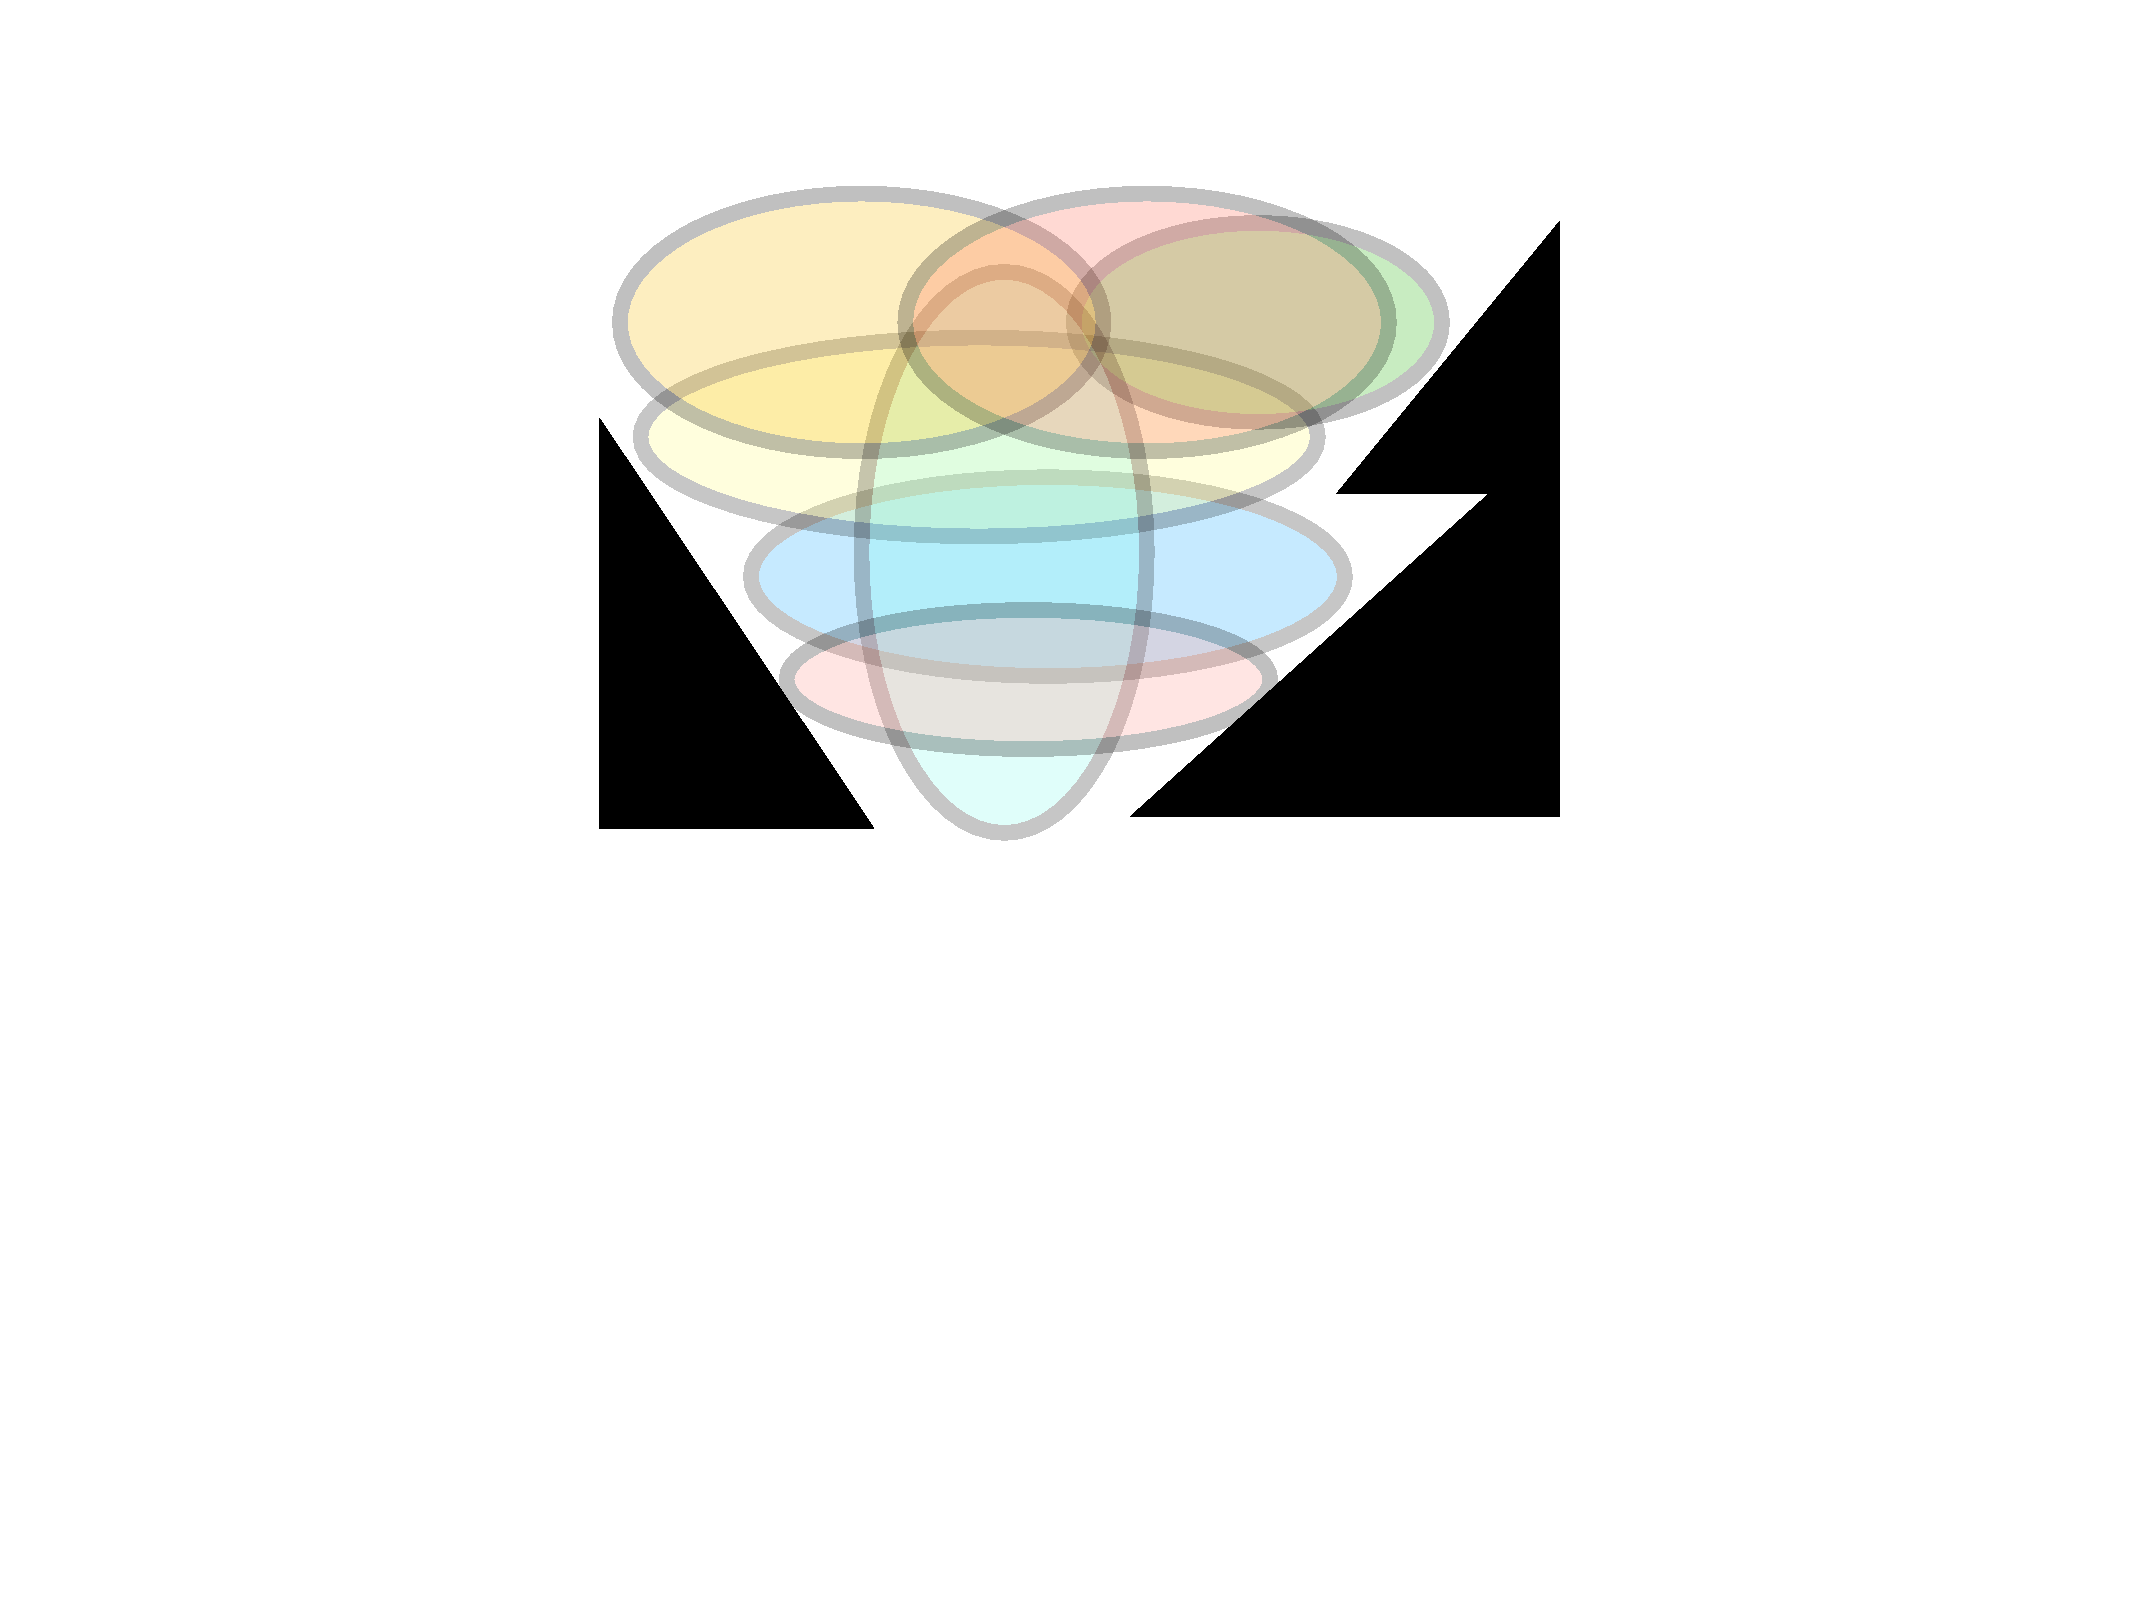
\includegraphics[width=\linewidth, trim=250  320 260 60,clip]{diagrams/NecAndSuff.pdf}
\end{minipage}
\\
sufficient  spec.& & necessary spec. & & holisitic spec.
%\begin{minipage}{0.75\textwidth}
%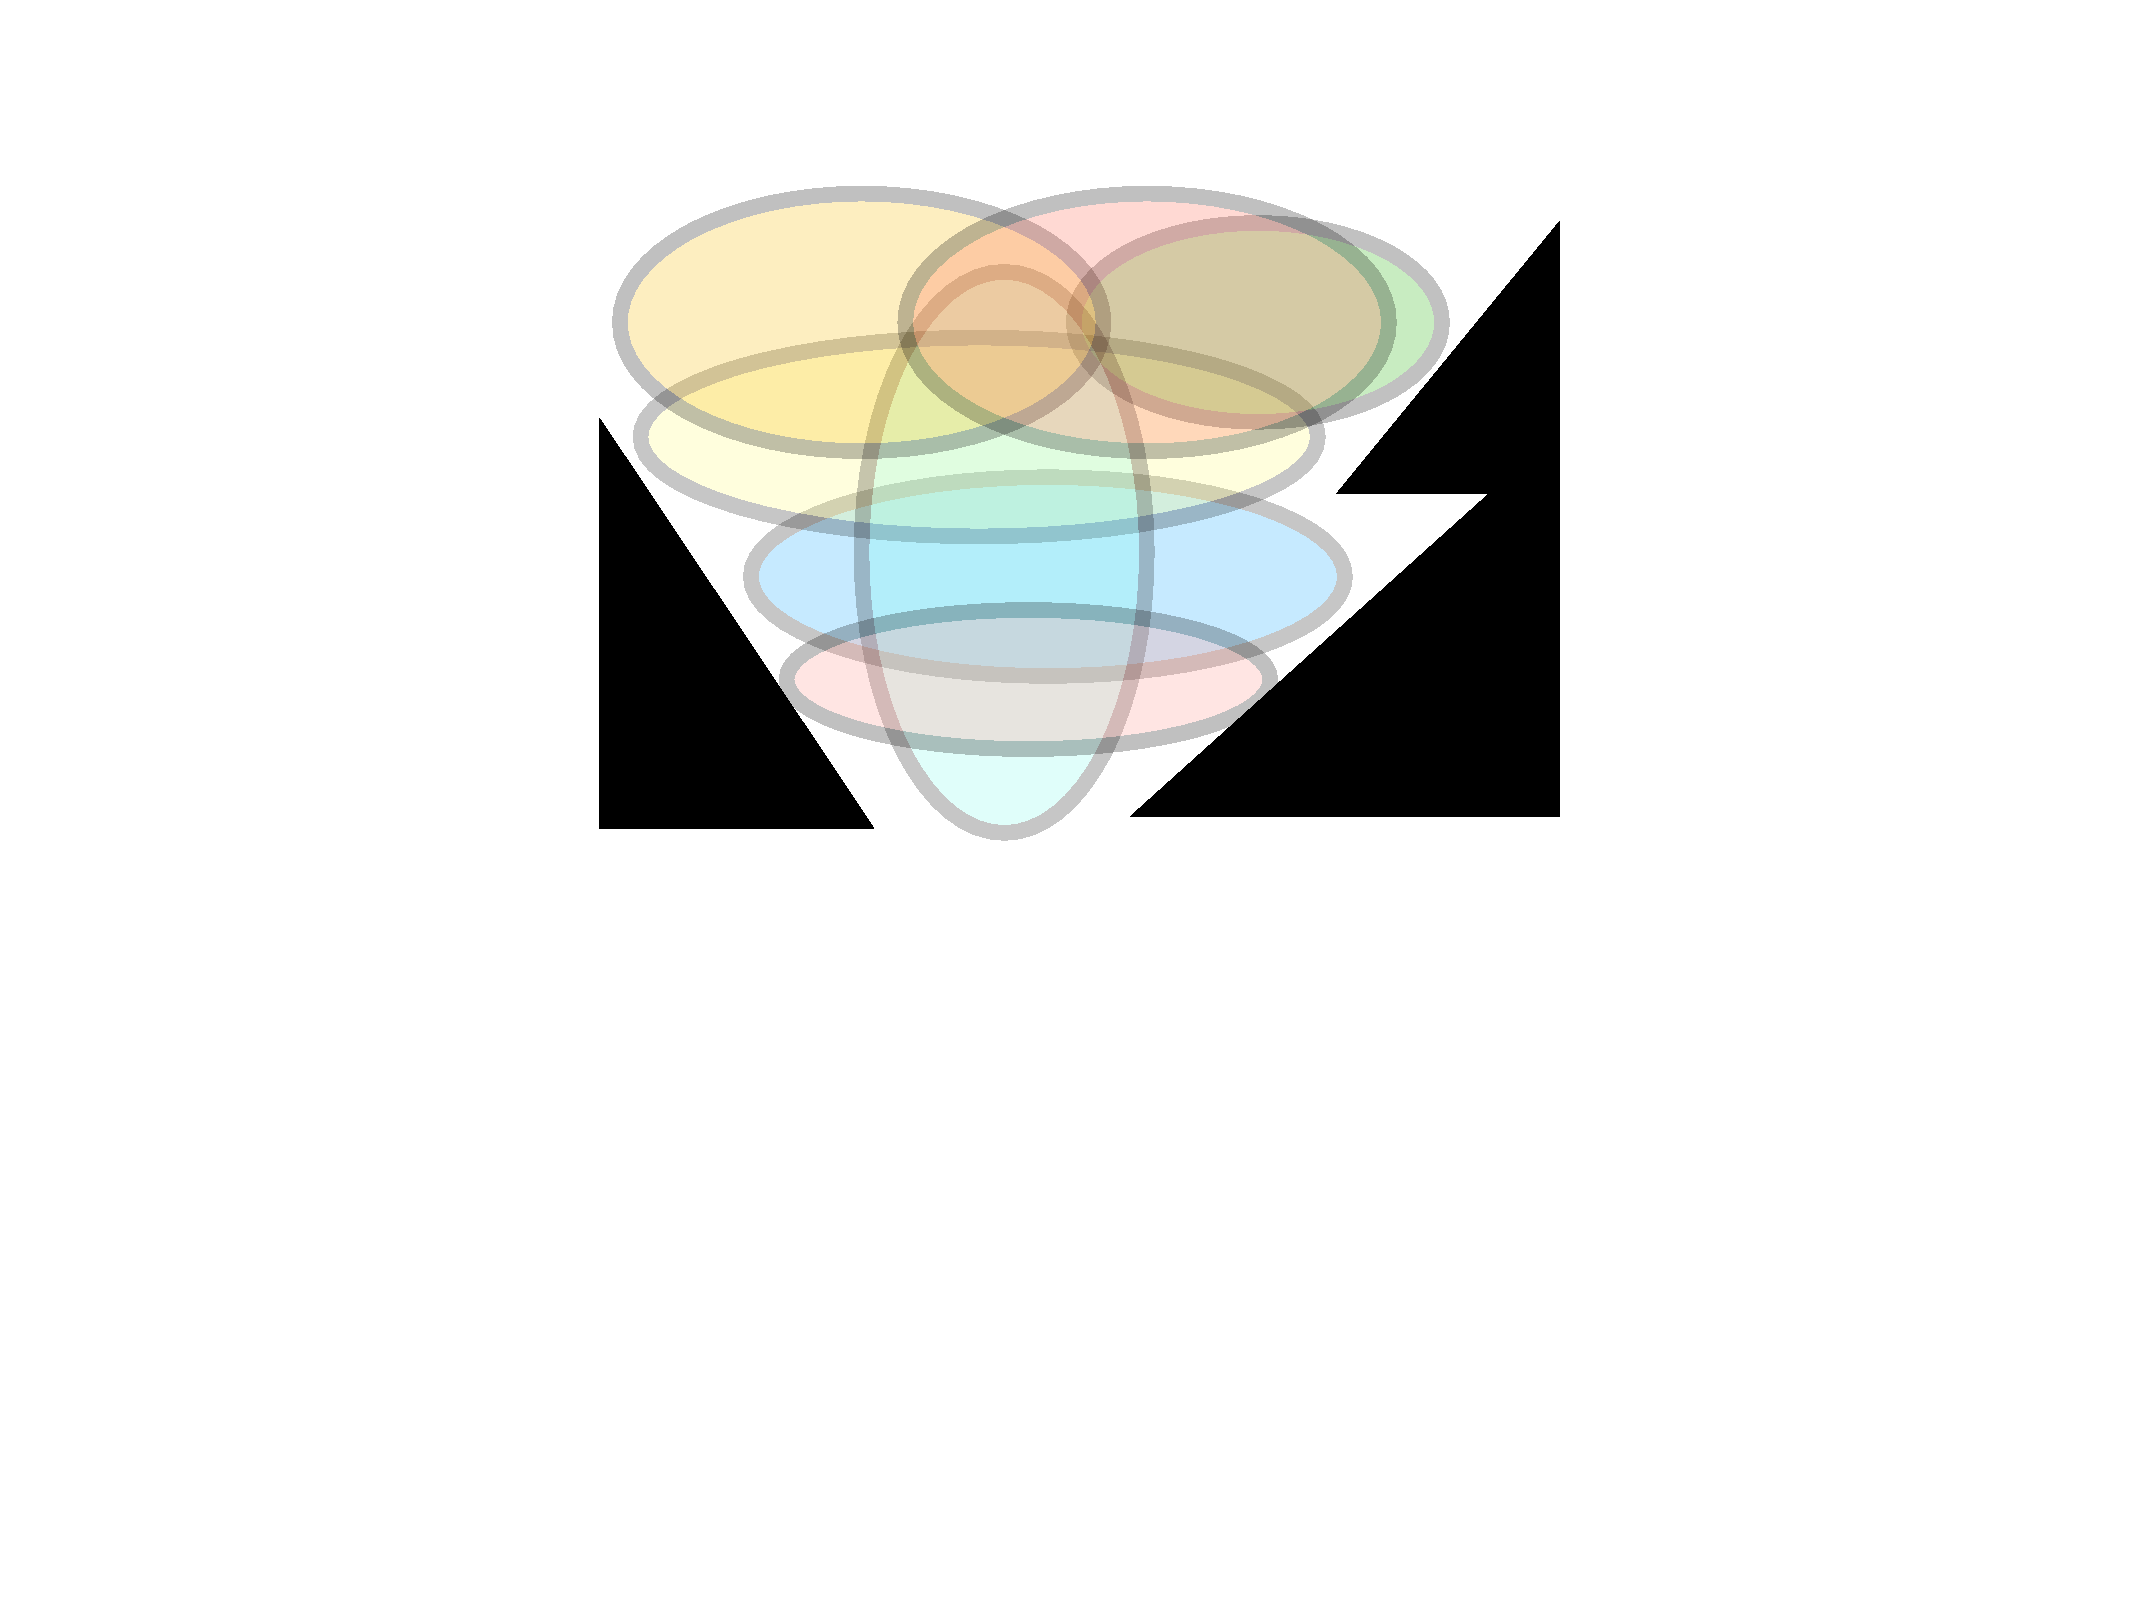
\includegraphics[width=\linewidth, trim=145  320 60 105,clip]{diagrams/NecAndSuff.pdf}
%\end{minipage}
%% y seems to eat up the bollom
%% x eats space from left, if you increase it the diagram decreases from left
%% w eats space from top, if you increase it the diagram decreases from top
%%\includegraphics[page=3, width=\linewidth, trim=150  270 40 150, clip]{diagrams/snmalloc.pdf}\sdcomment{I think we need to change the diagram so that it says small slab.}
%\end{minipage}
 \end{tabular}
  \vspace*{-2.5mm}
  \caption{Sufficient and Necessary Conditions, and Full Specifications}
 \label{fig:NecessaryAndSuff}
 \end{figure}
 
 We propose that  necessary conditions should be explicitly stated. Specifications should be \emph{holistic}, in the sense that they describe the  overall behaviour of a module: not only the behaviour  of each function separately, but also 
 emerging behaviours through combination of functions.
% Necessary conditions are  depicted by the black
% triangles in the middle  diagram in Fig \ref{fig:NecessaryAndSuff}.
A holistic specification should therefore consist of   the sufficient as well as the necessary conditions, as  
depicted in right hand side  diagram in Fig. \ref{fig:NecessaryAndSuff}.
In Section \ref{sec:discussion} we argue why necessary conditions are more than the complement of
sufficient conditions.

Necessary conditions are guarantees upheld throughout program execution.
Other systems which give such ``permanent'' guarantees are    type systems, 
which ensure that well-formed programs  always produce well-formed runtime
configurations, or information flow control systems \cite{infoflow}, which ensure that values 
classified as high  will not be passed into contexts classified as low. 
Such  guarantees %made by types or information flow control
 are  practical to check, but   too coarse grained
for the purpose of fine-grained,  module-specific specifications. 

Necessary conditions are  akin to  monitor or object invariants\cite{Hoare74,Meyer97}. The difference between
these and our holistic specifications is that object/monitor invariants can only reflect about 
the current state (\ie the contents of the
stack frame and the heap), while   holistic specifications reflect about all aspects of execution.

In this paper we propose \Chainmail, a specification language to express holistic specifications. \Chainmail extends 
traditional program specification languages\cite{jml,Eiffel}, with features which talk about

\begin{description}
\item[Permission] Which object may have access to which other objects. 
Accessibility is central since access to an object usually also grants access to the functions it provides.

\item[Control] What object called functions on other objects. This is useful in identifying the causes of certain effects - eg 
funds can only be reduced if the owner called a payment function.

\item[Authority]  Which objects' state or properties may change. This is useful in describing effects, such as  reduction of funds.

\item[Space] This is about which parts of the heap are considered when establishing some property, or when 
performing program execution. 
Related to, but different from memory footprints and separation logics.

\item[Time] Assertions about the past or the future.
\end{description}


The design of \Chainmail was guided by the study of a sequence of examples from the OCAP literature and the 
smart contracts world: the membrane, the DOM, the Mint/Purse, the Escrow, the DAO and ERC20. 
We were satisfied to see that the same concepts were used to specify examples from  different contexts.
Holistic assertions often have the form of a guarnantee
 that if some property ever hods in the future then some other property holds now.
For example, if within a certain heap some change is possible in the future, then this particular heap contains 
at least one object which has access to a specific other, privileged object.
%
While many individual features of \Chainmail can be found also in other work, 
we argue that their power and novelty for specifying open systems lies in their careful combination.
\sdcomment{ I think that James does not like this sentence. What could we say instead? Also, we need to
stress that the selection of these features was not arbitrary.}
 
A module satisfies such a holistic assertion if, for all other modules,
  the assertion is satisfied  in all runtime configurations reachable through execution of the two modules combined.
  This reflects the open-world view.
  
The contributions of this paper are
\begin{itemize}
\item The design of the holistic specification language \Chainmail,
\item The semantics of \Chainmail,
\item A validation of \Chainmail through its application to a sequence of examples,
\item A further validation of \Chainmail through informal proofs of adherence of code to some of these specifications
\end{itemize}  
  
  
The rest of the paper is organized as follows: Section~\ref{sect:mitave:DOM} 
motivates our work in terms of an example. Sections~\ref{sect:LangOO}-\ref{sect:assertions} contain a formal definition of of \LangOO, and the semantics of assertions. Section ... related work .... Section xxxx concludes.

  
   

 

 
%However what has been less well-studied
%so far, is the characterization of the ways in which a system is robust, \ie how do we
%specify robustness. What exactly do we expect from a module in 
%
% 
%The traditional (philosophically, the ``modern'' approach) to
%construct secure systems is to build up trusted components as an
%hierarchy on top of a known and trusted secured computing base,
%underpinned by verified and verifying compilers \cite{HoareManifesto}.
%This approach relies on a closed world assumption: there is an
%explicitly demarcated border between the inside and the outside of the
%system, and the whole system can be trusted because (and as long as)
%each component inside the border can be trusted. Similarly, each
%module is an independent demesnes \cite{wills}, jealously
%protecting its own invariants behind its own borders, giving rise to a
%series of layers of trust, layered virtual machines
%\cite{nosp} or protection rings \cite{pola}.
%
%Open
%systems, on the other hand, have an open world assumption: they must
%interact with a wide range of component objects with different levels
%of mutual trust (or distrust) --- and whose configuration dynamically
%changes.
%%
%% Consider electronic payments systems such as Swift, Paypal,
%% or WeSwap.com: they must transfer funds between participants'
%% accounts, where the participants do not trust each other, cannot be
%% trusted by the payments system, and may join or leave the system at
%% any time.  With multiple competing payments systems across different
%% international juristidctions, there is no central authority that can
%% vouch for the trusworthiness of participants or payments systems.
%%
%Given a method request \lstinline+x.m(y)+, what can
%we conclude about the behaviour of this request if we know nothing
%about the receiver \lstinline+x+?
% 
%
%The critical
%problem with building systems for an open world is that the actual
%invariants that must be maintained by a program will be
%\textit{implicit}, scattered throughout the program's modules.  Any
%part of a program that uses an object from a trusted module may (by
%oversight, error, or fraud) hand that object to an untrustworthy
%module, giving potentially malicious code access to all the services
%provided by the trustworthy module \cite{geneva91,aliasingBook}.  This
%makes it hard to determine what invariants are actually maintained by
%a given module, and thus verify the integrity of the overall system.
%%
%Miller \cite{miller-esop2013,MillerPhD} defines the necessary approach
%as \textbf{defensive consistency}: \textit{``An object is defensively
%  consistent when it can defend its own invariants and provide correct
%  service to its well behaved clients, despite arbitrary or malicious
%  misbehaviour by its other clients.''}  Defensively consistent
%modules are particularly hard to design, to write, to understand, and
%to verify: but they have the great advantage that they make it much
%easier to make guarantees about systems composed of multiple components
%\cite{Murray:phd}.
%
%
%In this paper, we present a modular specification language,
%\Chainmail, that is designed to support defensively consistent
%specifications of these kinds of open
%systems. Building on the object-capability model \cite{Elang},
%\Chainmail\ specifications are modular, as separate concerns in a
%system can be captured in as individual specification or policy
%definitions.  \Chainmail\ specifications 
%not tied to any particular module in a system but can define
%the behaviour of any complying module, and can cross-cut multiple
%modules.  \Chainmail\ policies define not only method pre- and post-
%conditions, but also give invariants that must be maintained
%\emph{irrespective} of any other code in the system, even when the
%actual composition of the system is unknown.  Taken together, this
%means that \Chainmail\ can specify modules that must be
%\emph{defensively consistent}, guaranteeing their integrity in an
%arbitrary open world.
%  
% 
%%\kjx{need to say what the case studies are.   or not!}
%
%
%%%%%%%%%%%%%%%%%%%%%%%%%%%%%%%%%%%%%%%%%%%%%%%%%%%%%%%%%%%%%
%%%% TO HERE
%%%%%%%%%%%%%%%%%%%%%%%%%%%%%%%%%%%%%%%%%%%%%%%%%%%%%%%%%%%%%
%
%
%\paragraph{Contribution} 
%This paper extends earlier informal work mostly presented at
%workshops~\cite{capeFTfJP,capeFTfJP14,swapsiesOnTheInternet2015,capeIFM14}.
%Here we present the full design of \Chainmail\ for the first time, and
%show how \Chainmail\ allows us to write modular, multi-dimensional
%specifications for the open world.  As is traditional, some details
%are relegated to a technical report~\cite{appendix}.
%
%To address the open nature of the systems, we make the meaning of
%policies parametric with any code that may be linked to the
%current system.  We give examples to show how \Chainmail\ modules can
%be written in a very robust, defensively consistent manner, so that no
%further, malicious code can steal their secrets or break their
%integrity.
%
%% This has let us give a
%% formal meaning to Miller's \emph{defensive consistency} for the first
%% time. \tobym{Not quite true. I had a stab at defining defensive correctness
%% and consistency in my PhD thesis, which I've summarised in \autoref{sec:related}.}
%
%Our design of \Chainmail\ is part of a larger research project about
%specifying and verifying systems in an open world.  Security is of
%particular concern in open systems, and \Chainmail\ includes
%assertions such as (\obeys, \MayAffect, and \MayAccess) to allow
%us to reason explicitly about module's security properties and
%guarantees.  Elsewhere we demonstrate how these constructs let us
%describe how components can co{\"o}perate to establish trust
%gradually, and to delineate the risks involved in that co{\"o}peration
%\cite{POSTSUBMITTED}. Security, trust, and risk are not the focus of
%this paper, rather here we concentrate on the core features of
%\Chainmail, showing how \Chainmail\ policies permit modular,
%defensively consistent specifications.
%
%To give a semantics to \Chainmail\ policies we have also defined a
%core object-oriented programming language, \LangOO, (the Featherweight
%Object Capability Language, not to be confused with FOCAL
%\cite{FOCAL-69}), described in more detail elsewhere \cite{appendix}.
%\LangOO\ is a simple, dynamically typed language with traditional
%classes as its modularly mechanism.  That is, \Chainmail\ provides
%separation of concerns for \emph{specifications} of object-oriented
%\emph{implementations}.  We made this design choice for several
%reasons, primarily because we are interested in specifications, rather
%than implementations.  We are primarily
%interested in specifying ``real world'' programs, which tend to be
%written in OO languages like JavaScript, Java or E, rather than e.g.\
%aspect- or subject- oriented languages; and that we wanted to keep
%\LangOO\ as simple as possible.  We hope to extend our specification
%techniques to more modular languages in future work.
%
%To prove a program's adherence to \Chainmail\ specifications, we have
%developed a Hoare logic and associated inference rules.  We do not
%discuss the logic or these rules in this paper, although they are
%present in the technical report \cite{appendix}.
 
